% version 1.00, date 30/11/16, auteur Kafui Atanley
\section{Lot 3}
	Le lot 3 devra faire état de cinq fonctionnalités additionnelles. Il devra être impérativement livré au client avant le vendredi 9 décembre 2016. \\
	
	La figure \ref{fonctPrinc} montre l’interaction entre les différentes fonctionnalités à l'aide d'un diagramme de séquence UML.

\begin{figure}[H]
	\begin{center}
	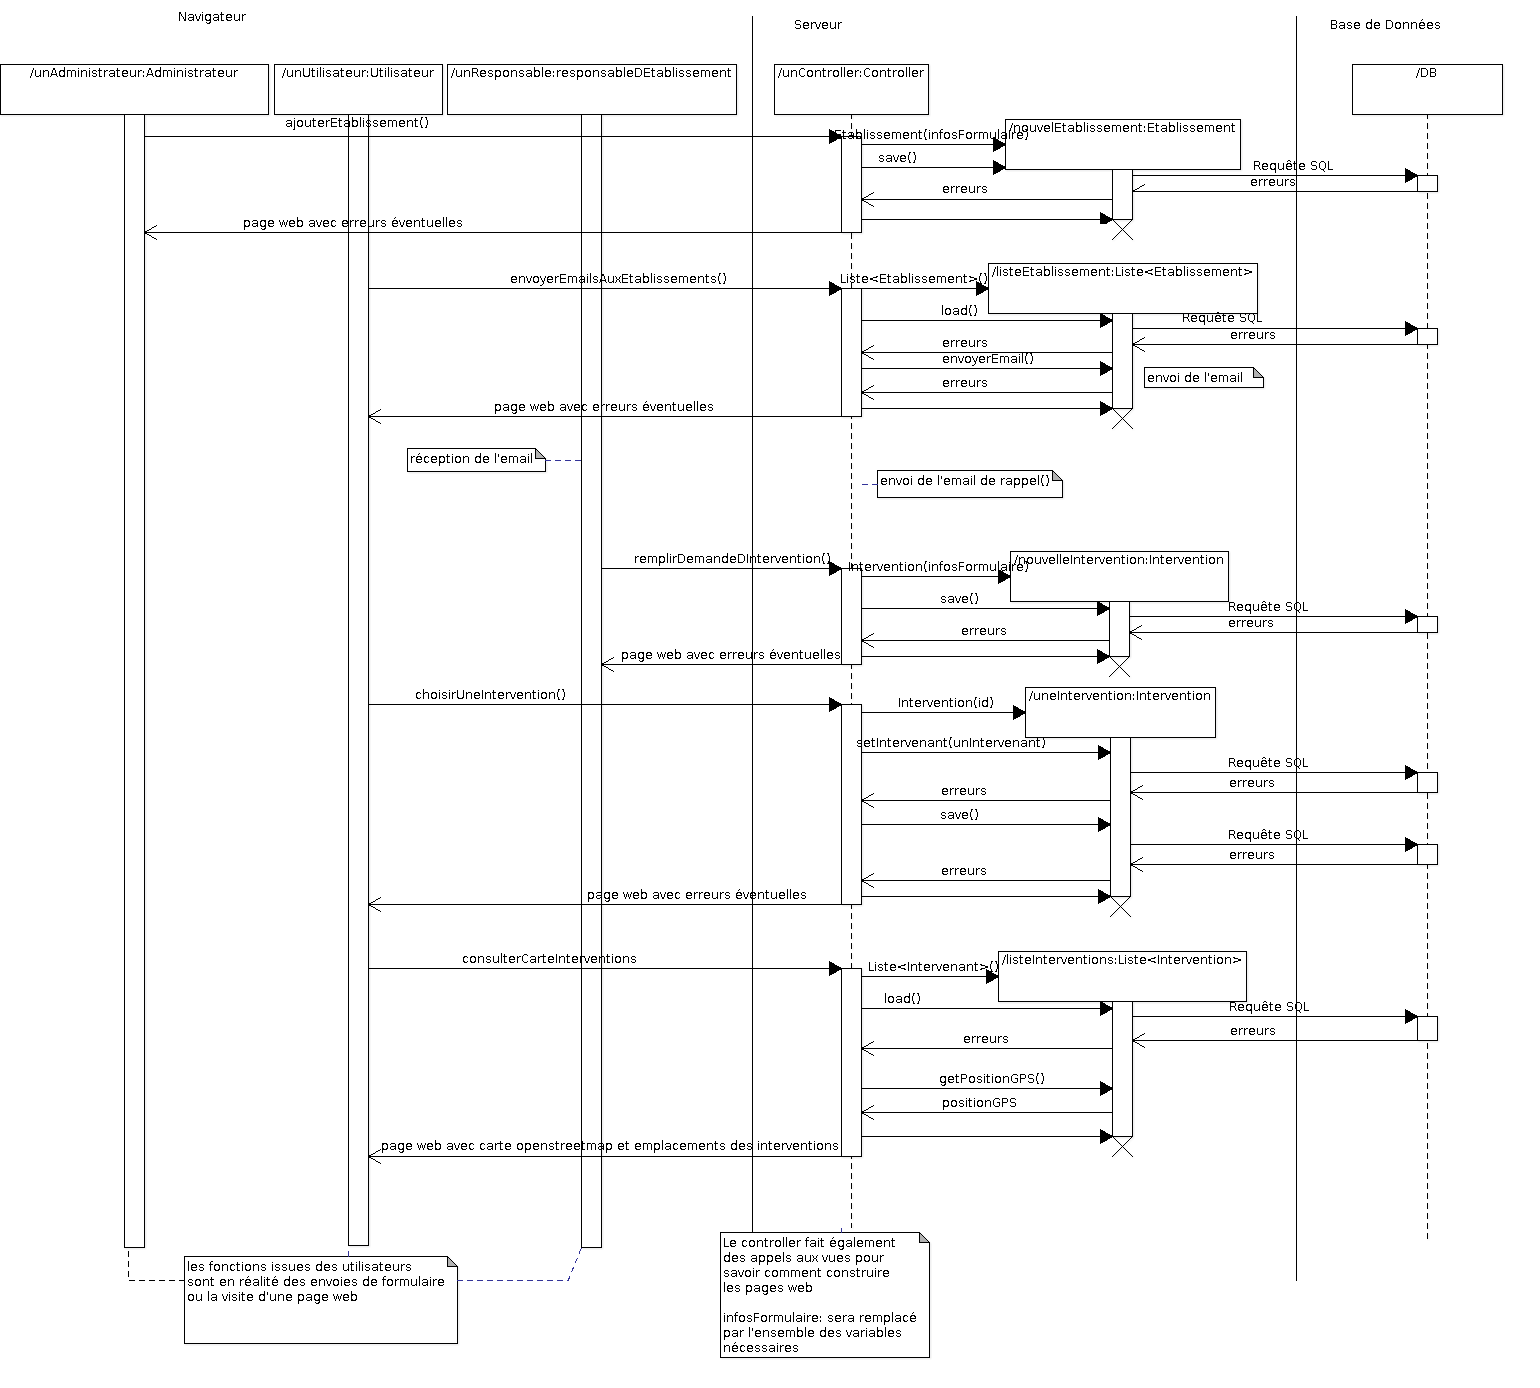
\includegraphics[scale=0.3]{images/fonctionsPrincipales.png}
	\caption{\label{fonctPrinc} Diagramme de séquence représentant les fonctions principales du logiciel}
	\end{center}
\end{figure}

% version 1.00, date 05/11/16, auteur Kafui Atanley
\subsection{Fonctionnalité 8}
La fonctionnalité 7 permettra d’envoyer un e-mail de rappel à l’établissement et au contact
dans l’établissement (si son adresse électronique est différente de celle de l’établissement),
une semaine avant l’intervention.


% version 1.00, date 05/11/16, auteur Kafui Atanley
%L’outil devra faciliter la géolocalisation des établissements, bénévoles et interventions.
%Une carte devra pouvoir être accessible quand l’une des entité possède une adresse et il
%devra être possible de filtrer ces entités en fonction de la distance à une ville ou un point
%géographique particulier à l’aide de liste.
\subsection{Fonctionnalité 9}

La fonctionnalité 9 concerne la géolocalisation des entités possédant une adresse.
Ces entités sont : 
\begin{itemize}
\item les établissements,
\item les interventions quelque soit leur type,
\item les ventes.
\end{itemize}
Une carte devra être affichée dans les fiches détaillées de chaque entité.
La maquette \ref{fonctionnalite9Geolocalisation} présente la fiche descriptive d'une entité. Les fiches descriptives
des entités interventions et ventes devront comporter une carte de manière similaire.
Il devra être possible de filtrer ces entités selon une ville et selon la distance par rapport à une ville.
La maquette \ref{fonctionnalite9Filtre} présente un modèle des filtres attendus sur les entités concernées.

\begin{figure}[H]
	\centering
	\includegraphics[scale=0.4]{images/maquettes/fonctionnalite9Geolocalisation.png}
	 \caption{Maquette~: Géolocalisation dans les fiches descriptives}
	 \label{fonctionnalite9Geolocalisation}
\end{figure}

\begin{figure}[H]
	\centering
	\includegraphics[scale=0.4]{images/maquettes/fonctionnalite9Filtre.png}
	 \caption{Maquette~: Modèle de filtres attendus}
	 \label{fonctionnalite9Filtre}
\end{figure}


% version 1.00, date 05/11/16, auteur Kafui Atanley
\subsection{Fonctionnalité 10}




